\documentclass[12pt]{article}
\pagenumbering{gobble}
\linespread{1.1}

\usepackage{amsfonts}
\usepackage{amsmath}
\usepackage{amssymb}
\usepackage{array}
\usepackage{fancyhdr}
\usepackage{mathrsfs}
\usepackage{mathtools}
\usepackage{parskip}
\usepackage{textcomp}
\usepackage[margin=1in,headheight=1in]{geometry}

\usepackage{tikz}
\usetikzlibrary{animations}
\usetikzlibrary{arrows.meta}
\usetikzlibrary{calc}
\usetikzlibrary{shapes.geometric}
\usetikzlibrary{positioning}

\tikzset{label/.style={draw=black}}
\tikzset{arrow/.style={-stealth,shorten >= 1mm}}

\newcommand{\contradiction}{
    \ensuremath{{\Rightarrow\mspace{-2mu}\Leftarrow}}
}

% bracket commands
\newcommand{\angleb}[1]{\left\langle#1\right\rangle} % <>
\newcommand{\vertb}[1]{\left\vert#1\right\vert}      % ||
\newcommand{\bracks}[1]{\left[#1\right]}             % []
\newcommand{\braces}[1]{\left\{#1\right\}}           % {}
\newcommand{\parens}[1]{\left(#1\right)}             % ()

% set aliases
\newcommand{\N}{\mathbb{N}}
\newcommand{\Z}{\mathbb{Z}}
\newcommand{\Q}{\mathbb{Q}}
\newcommand{\R}{\mathbb{R}}

\newcommand{\derv}[2]{\dfrac{d#1}{d#2}}
\newcommand{\e}{\varepsilon}
\newcommand{\lm}[1]{\displaystyle\lim_{#1}}

% tikz
\newcommand{\dframe}{
    \draw[rounded corners] (-8,3) rectangle (8,-3);
}

\begin{document}

\pagestyle{fancy}
\fancyhead[L]{Alex Agruso}
\fancyhead[R]{Topology Writing 12}

I can't make this one connected graph due to a lack of space, so assume that
two nodes of the same name represent the same vertex in the whole graph, just
with certain surrounding vertices omitted depending on the section.

\begin{center}
	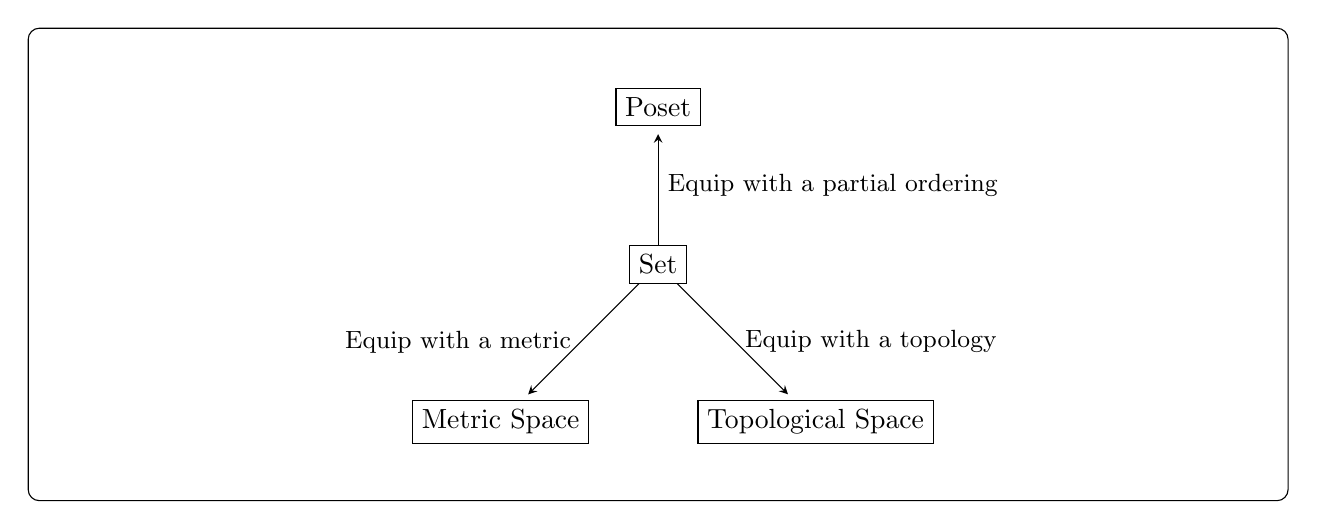
\begin{tikzpicture}
        \dframe

        \node[label] (set) at (0,0) {Set};
        \node[label] (pos) at (0,2) {Poset};
        \node[label] (tsp) at (2,-2) {Topological Space};
        \node[label] (msp) at (-2,-2) {Metric Space};

        \draw[->, arrow] (set) -- (tsp) node[midway,right]
            {\small Equip with a topology};
        \draw[->, arrow] (set) -- (msp) node[midway,left]
            {\small Equip with a metric};
        \draw[->, arrow] (set) -- (pos) node[midway,right]
            {\small Equip with a partial ordering};
	\end{tikzpicture}

	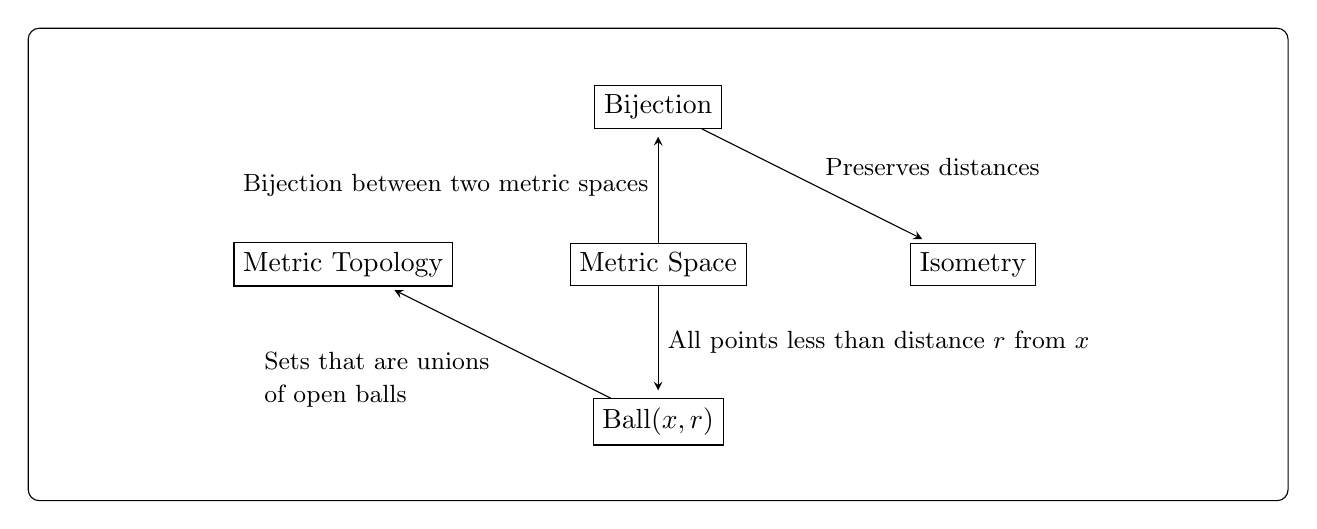
\begin{tikzpicture}
        \dframe

        \node[label] (msp) at (0,0) {Metric Space};
        \node[label] (bij) at (0,2) {Bijection};
        \node[label] (opb) at (0,-2) {Ball$(x,r)$};
        \node[label] (mtp) at (-4,0) {Metric Topology};
        \node[label] (iso) at (4,0) {Isometry};

        \draw[->, arrow] (msp) -- (bij) node [midway,left]
            {\small Bijection between two metric spaces};
        \draw[->, arrow] (bij) -- (iso) node [midway,above right]
            {\small Preserves distances};
        \draw[->, arrow] (msp) -- (opb) node [midway,right]
            {\small All points less than distance $r$ from $x$};
        \draw[arrow] (opb) -- (mtp) node [midway,below left,align=left]
            {\small Sets that are unions\\
            \small of open balls};
	\end{tikzpicture}

    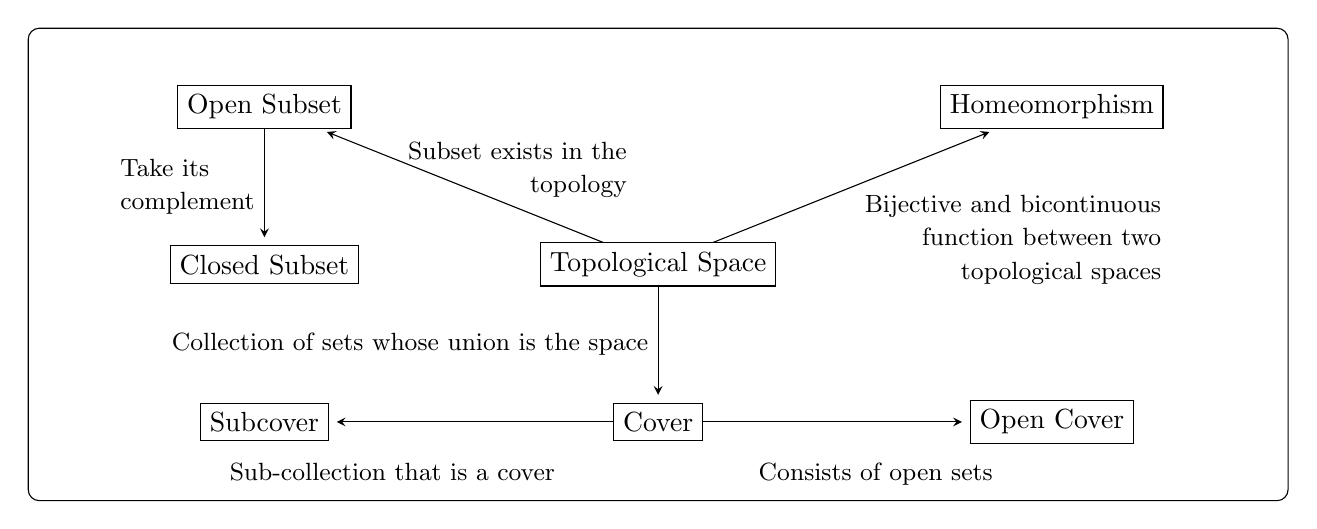
\begin{tikzpicture}
        \dframe

        \node[label] (tsp) at (0,0) {Topological Space};
        \node[label] (hme) at (5,2) {Homeomorphism};
        \node[label] (cvr) at (0,-2) {Cover};
        \node[label] (ocv) at (5,-2) {Open Cover};
        \node[label] (scv) at (-5,-2) {Subcover};
        \node[label] (osb) at (-5,2) {Open Subset};
        \node[label] (csb) at (-5,0) {Closed Subset};

        \draw[arrow] (tsp) -- (hme) node[midway,below right,align=right]
            {\small Bijective and bicontinuous\\
                \small function between two\\
                \small topological spaces};
        \draw[arrow] (tsp) -- (cvr) node[midway,left]
            {\small Collection of sets whose union is the space};
        \draw[arrow] (cvr) -- (ocv) node[midway,below,yshift=-4mm,xshift=5mm]
            {\small Consists of open sets};
        \draw[arrow] (cvr) -- (scv) node[midway,below,yshift=-4mm,xshift=-10mm]
            {\small Sub-collection that is a cover};
        \draw[arrow] (tsp) -- (osb)
            node[midway,right,xshift=-8mm,yshift=2mm,align=right]
            {\small Subset exists in the\\
                \small topology};
        \draw[arrow] (osb) -- (csb) node[midway,left,align=left]
            {\small Take its\\
                \small complement};
    \end{tikzpicture}

    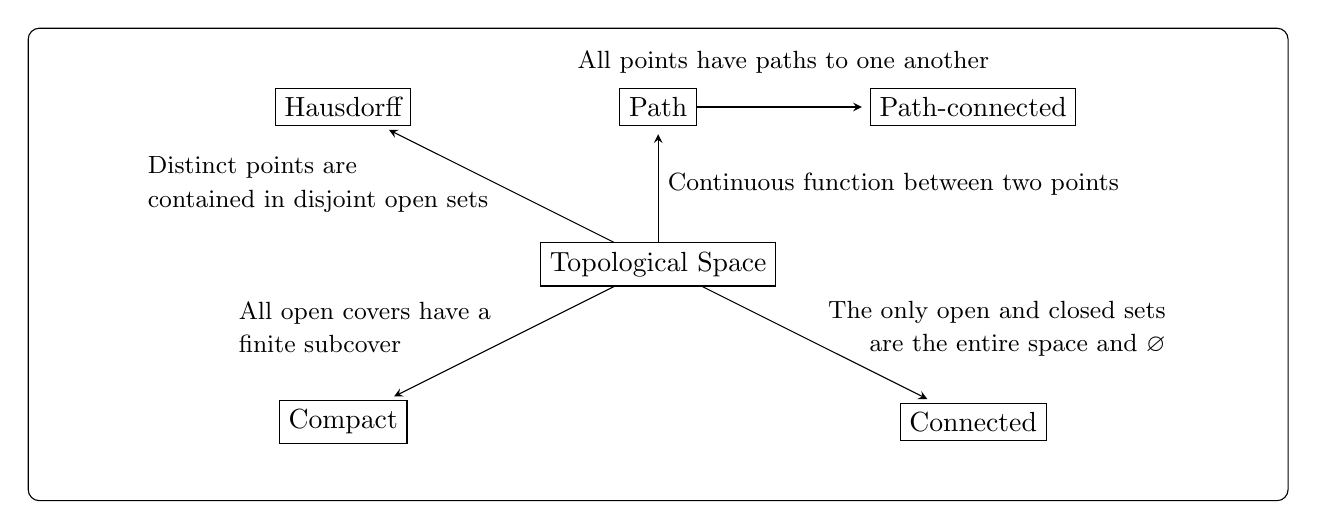
\begin{tikzpicture}
        \dframe

        \node[label] (tsp) at (0,0) {Topological Space};
        \node[label] (hsd) at (-4,2) {Hausdorff};
        \node[label] (cmp) at (-4,-2) {Compact};
        \node[label] (con) at (4,-2) {Connected};
        \node[label] (pth) at (0,2) {Path};
        \node[label] (ptc) at (4,2) {Path-connected};

        \draw[->, arrow] (tsp) -- (hsd)
            node [midway,left,align=left]
            {\small Distinct points are\\
            \small contained in disjoint open sets};
        \draw[->, arrow] (tsp) -- (cmp)
            node [midway,left,align=left,yshift=2mm]
            {\small All open covers have a\\
            \small finite subcover};
        \draw[->, arrow] (tsp) -- (con)
            node [midway,right,align=right,yshift=2mm]
            {\small The only open and closed sets\\
            \small are the entire space and $\varnothing$};
        \draw[->, arrow] (tsp) -- (pth)
            node [midway,right]
            {\small Continuous function between two points};
        \draw[->, arrow] (pth) -- (ptc)
            node [midway,above,yshift=3mm]
            {\small All points have paths to one another};
    \end{tikzpicture}

    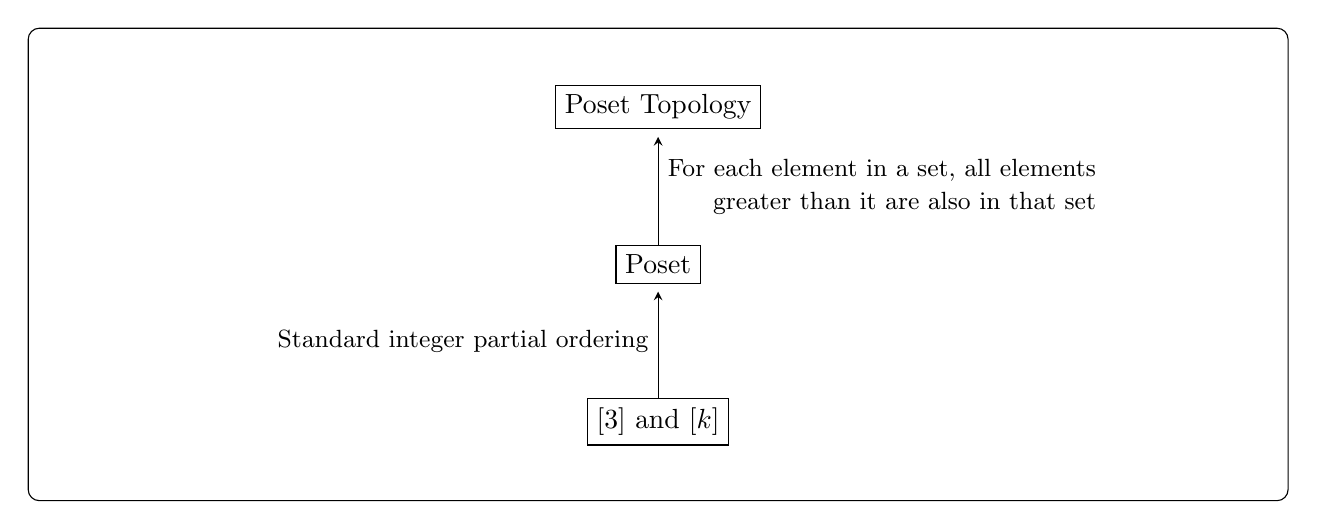
\begin{tikzpicture}
        \dframe

        \node[label] (pos) at (0,0) {Poset};
        \node[label] (exm) at (0,-2) {$[3]$ and $[k]$};
        \node[label] (alt) at (0,2) {Poset Topology};

        \draw[arrow] (exm) -- (pos) node[midway,left,align=left]
            {\small Standard integer partial ordering};
        \draw[arrow] (pos) -- (alt) node[midway,right,align=right]
            {\small For each element in a set, all elements \\
                \small greater than it are also in that set};
    \end{tikzpicture}
\end{center}

\end{document}
